\documentclass[10pt,twocolumn,letterpaper]{article}

\usepackage{cvpr}
\usepackage{times}
\usepackage{epsfig}
\usepackage{graphicx}
\usepackage{amsmath}
\usepackage{amssymb}
\usepackage{CJKutf8}
% Include other packages here, before hyperref.

% If you comment hyperref and then uncomment it, you should delete
% egpaper.aux before re-running latex.  (Or just hit 'q' on the first latex
% run, let it finish, and you should be clear).
\usepackage[breaklinks=true,bookmarks=false]{hyperref}

\cvprfinalcopy % *** Uncomment this line for the final submission

\def\cvprPaperID{****} % *** Enter the CVPR Paper ID here
\def\httilde{\mbox{\tt\raisebox{-.5ex}{\symbol{126}}}}

% Pages are numbered in submission mode, and unnumbered in camera-ready
%\ifcvprfinal\pagestyle{empty}\fi
\setcounter{page}{1}
\begin{document}
\begin{CJK}{UTF8}{bsmi}

%%%%%%%%% TITLE
\title{Auto Turn Sheet Music}

\author{林郁翔\\
P76094509\\
{\tt\small richardlin0212@gmail.com}
% For a paper whose authors are all at the same institution,
% omit the following lines up until the closing ``}''.
% Additional authors and addresses can be added with ``\and'',
% just like the second author.
% To save space, use either the email address or home page, not both
\and
方嘉祥\\
P76094151\\
{\tt\small frank870622@gmail.com}
}

\maketitle
%\thispagestyle{empty}

%%%%%%%%% ABSTRACT
\begin{abstract}
   For a song you played for the first time, you usually need to look at the sheet music to play, and most pile of sheet music are not only one page, so you must turn page when you are about to finish playing the page.

   We want to develop a software that can automatically scroll the guitar tablature with the progress of the music according to the input music or video.
\end{abstract}

%%%%%%%%% BODY TEXT
\section{Introduction}

Anyone who has experience in playing musical instruments knows that most musical instruments require both hands to play. 
Most pile of sheet music have more than one page, so when you are about to finish one page, you must turn a page. 
For paper-made sheet music, you can line up the papers without turning pages, but if you want to see all the sheet music on electronic scores, you must reduce the sheet music to a small size, and notes are too small to see.

%\begin{figure}[t]
%\begin{center}
   %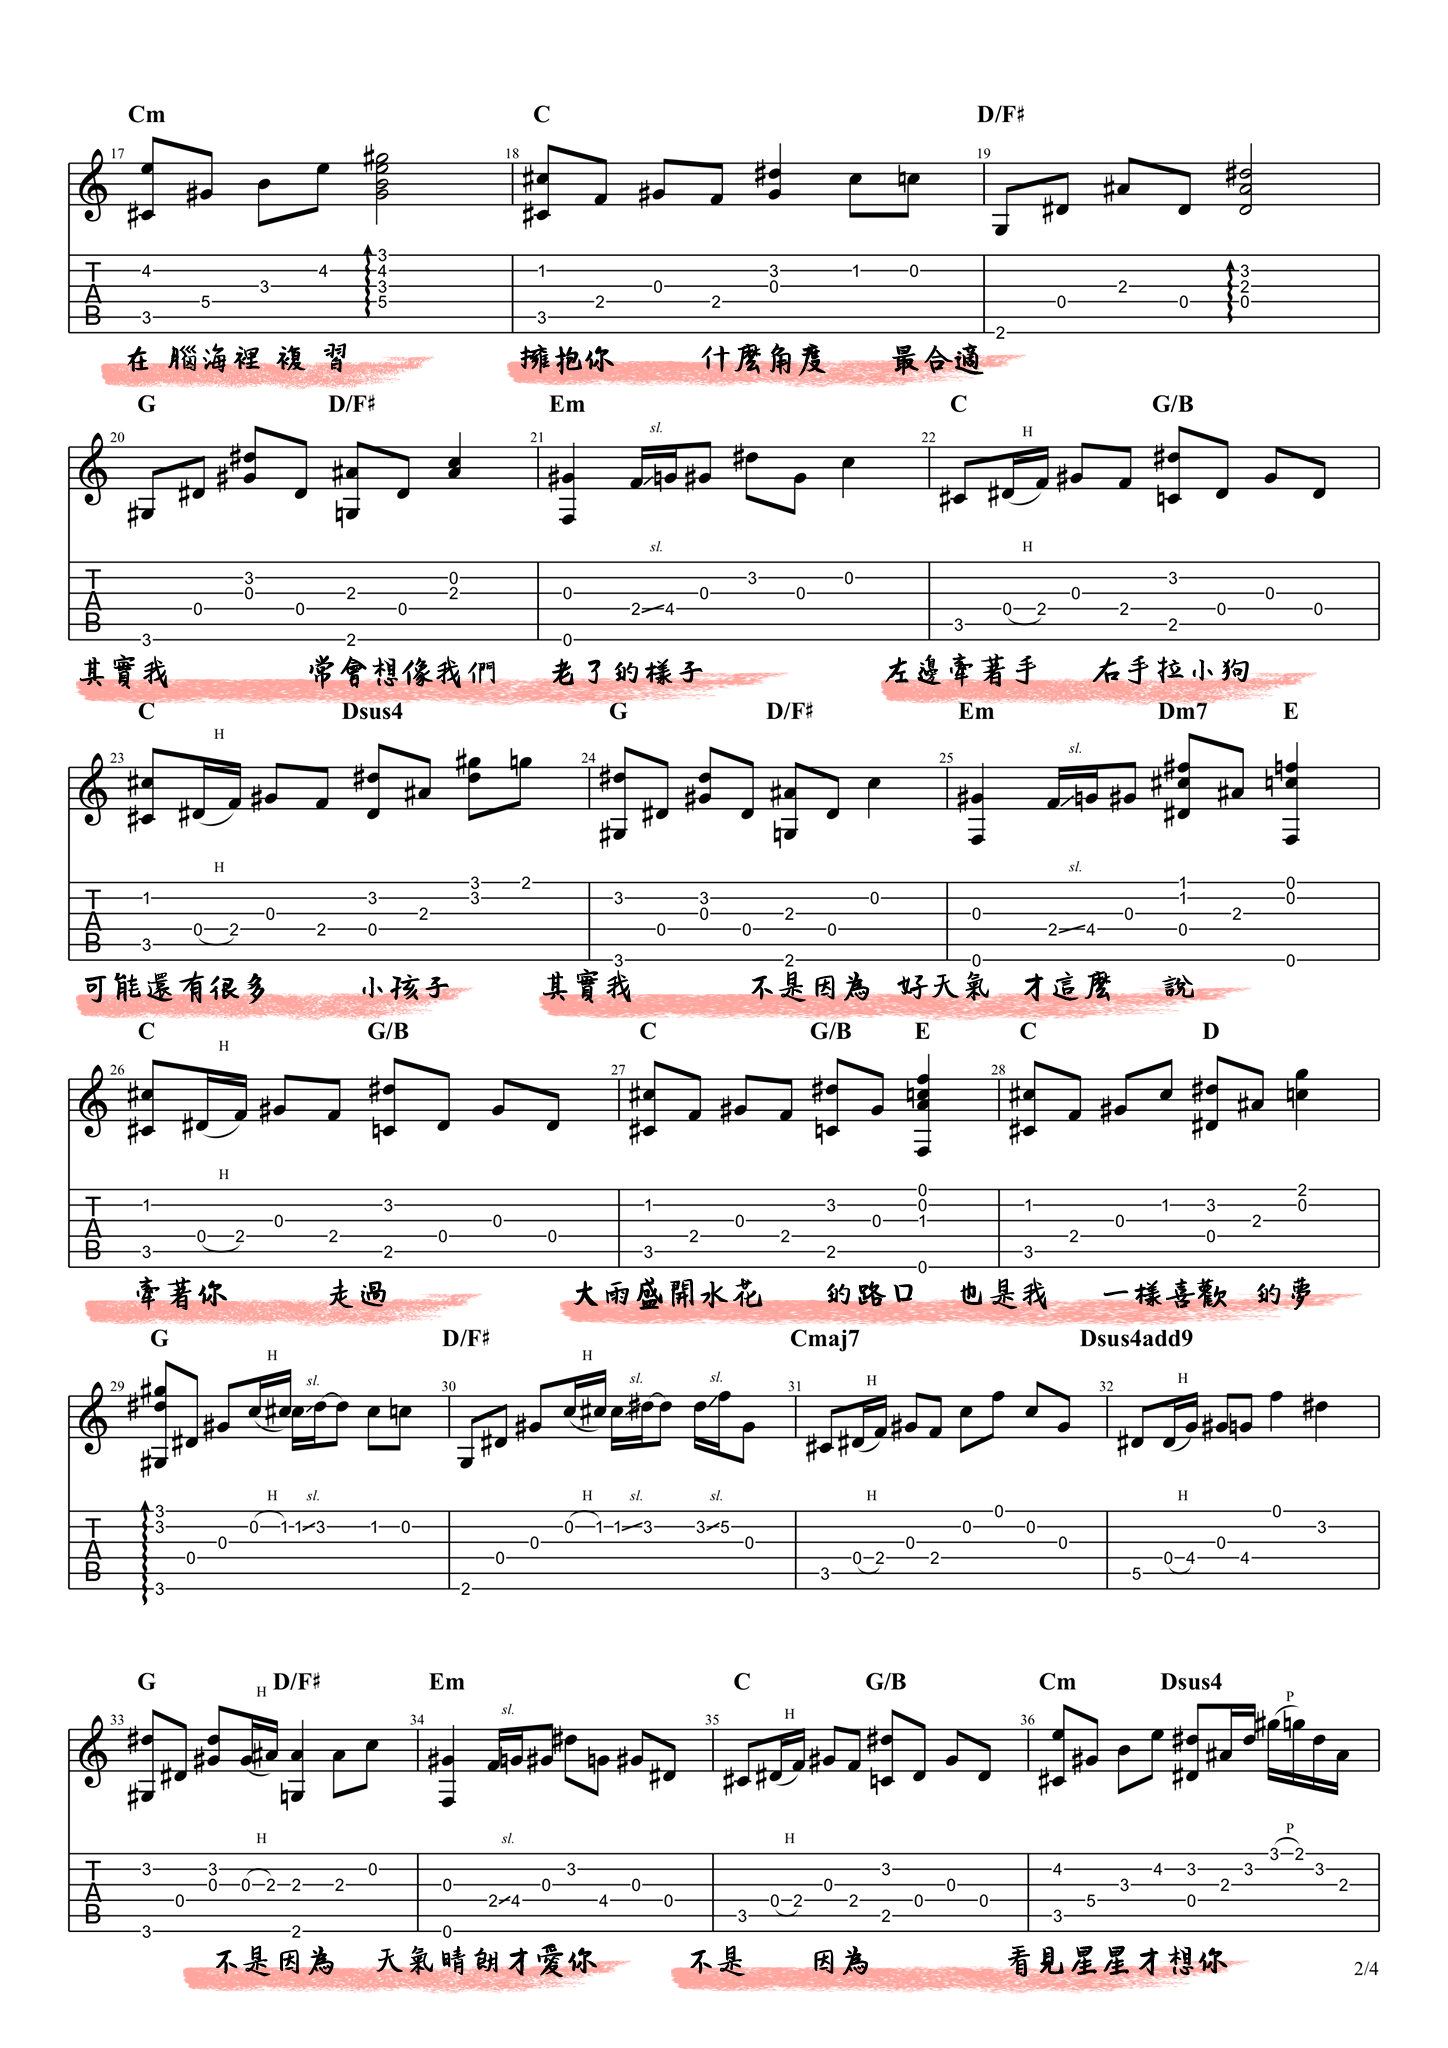
\includegraphics[width=0.8\linewidth]{2.png}
%\end{center}
   %\caption{Example of Guitar Tabs}
%\label{fig:long}
%\label{fig:guitar}
%\end{figure}

When practicing guitar, if it is not a self-created piece or a covered song, it is usually played with the existing music, usually a popular music film.
If you only list the chords, most of them don’t need to turn pages, but the guitar tabs that pay more attention to fingering are usually presented in the form of six-line tabs, tablatures, corresponding to the first to sixth strings of the guitar from top to bottom. 
Tablature may present in many aspects. 
It can come with five-line staff(Figure ~\ref{fig:tab1}), or show alone(Figure ~\ref{fig:tab2}). 
At this time, the number of tablature pages will rise quickly, and the number of times the sheet music will be flipped will also increase significantly. 
Also, if you are practicing against existing music, you will interrupt the practice when you turn the page. 
Or you want to focus on practicing a certain paragraph, you need to turn the sheet music to the position at the same time, and the music must be fixed to a certain place, which is a waste of time .

\begin{figure}[t]
\begin{center}
   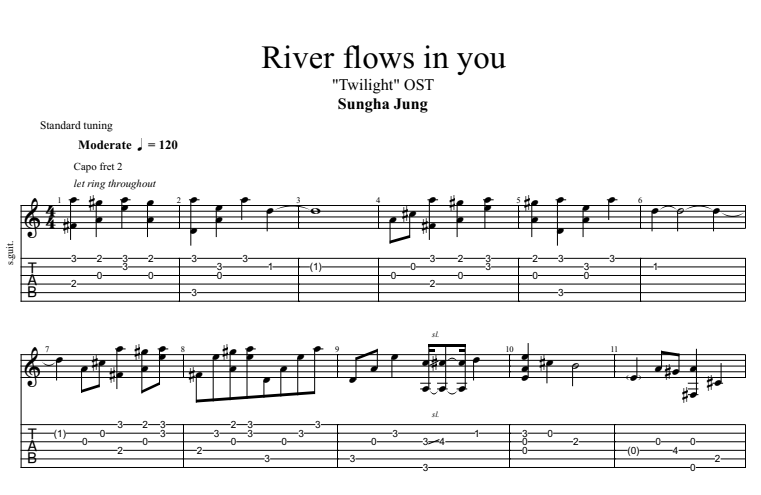
\includegraphics[width=0.9\linewidth]{tablature.png}
\end{center}
\caption{Example of Guitar Tabs with staff\cite{river_flows_in_you}}
\label{fig:long}
\label{fig:tab1}
\end{figure}

\begin{figure}[t]
\begin{center}
   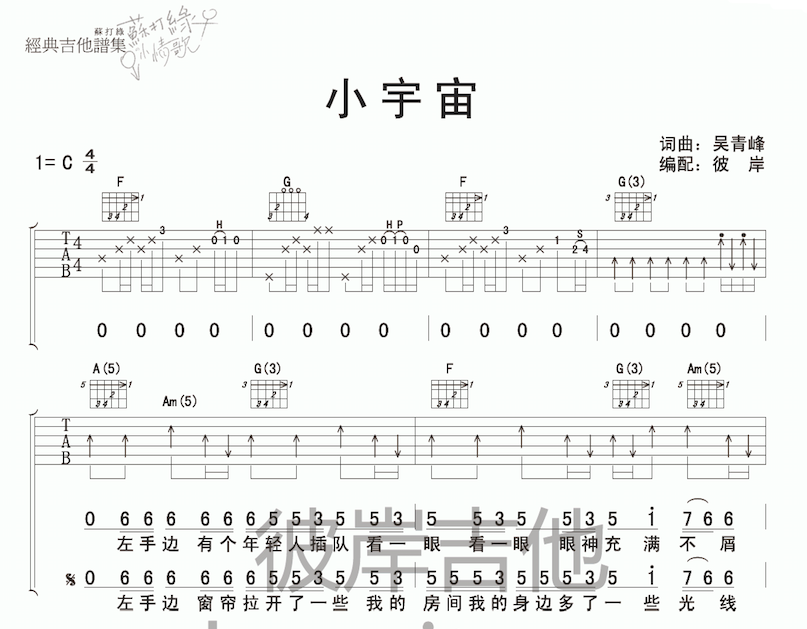
\includegraphics[width=0.9\linewidth]{tab2.png}
\end{center}
\caption{Example of Guitar Tabs without staff\cite{small_universe}}
\label{fig:long}
\label{fig:tab2}
\end{figure}

We want to develop a software that can automatically scroll the tablature with the progress of the music according to the input guitar music or video, and in conjunction with the input tablature.
Existing software requires a certain format (gp5, midi) to perform related work. 
We want to analyze the most common pdf and scroll the tablatures stored in the pdf according to the music. 
We also hope that users can pause the music at any time, or adjust the music to an appropriate position, and the tablature will also reach the correct paragraph.

%------------------------------------------------------------------------
\section{Related works}

\begin{figure}[t]
\begin{center}
   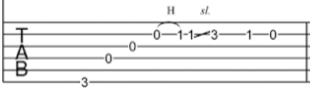
\includegraphics[width=0.8\linewidth]{relate_works_1.png}
\end{center}
    \caption{Six-line score}
\label{fig:relate_works_1}
\end{figure}

\begin{figure}[t]
\begin{center}
   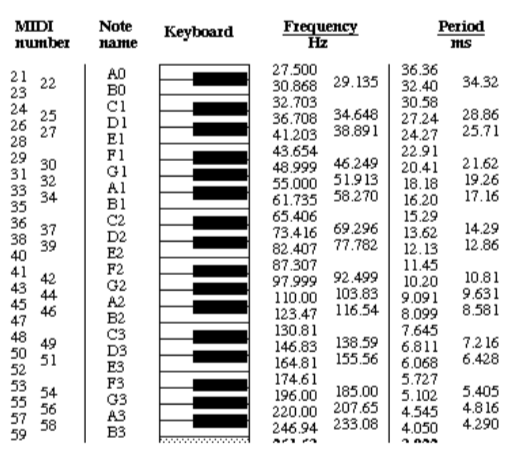
\includegraphics[width=0.8\linewidth]{relate_works_2.png}
\end{center}
   \caption{MIDI example\cite{midi_number}}
\label{fig:relate_works_2}
\end{figure}

A tablature is a kind of music score that records how a stringed instrument is played. In this case, from top to bottom, each line corresponds to the first to sixth strings of the guitar. The number on the line indicates the number of bars on the string to be played.(Figure ~\ref{fig:relate_works_1}).

MIDI numbers are a way to define notes by numbers, each semitone is regarded as a degree, A0 is 21, A\#0 is 22, and so on(Figure ~\ref{fig:relate_works_2}).

Optical Music Recognition (OMR), also named Music Optical Character Recognition, is a technology that converts music scores into a computer-readable format\cite{omr_survey}. Allows people to perform many operations with electronic music scores. In fact, there are already many people studying this technology. OMR has also progressed from computer vision recognition to deep learning.
Based on staff line of sheet music, \cite{staff_detection} tried to recognize hand-written sheet music.
\cite{expert_system} turned sheet music to guitar tablature. He not only recognize sheet music but also generate guitar tablature. 
A lot of people have tried to recognize staff, but few of them considered to recognize tablature.
So, we tried to recognize tablature.


%------------------------------------------------------------------------
\section{Method}

\subsection{Music score recognition method}
\begin{description}
\item 1. First we identify the position of the tablature.
\item 2. Then we identify each type of number once, and delete the out-of-range results by the position of the tablature we recognized.
\item 3. According to the ordering of notes on tablature, we sort all the numerical results found.
\item 4. We then identify the position of each line in the tablature, and mark which line and paragraph the number is on.
\item 5. Finally, we can know which page, row, and number each number is on.
\end{description}


\begin{figure}[t]
\begin{center}
   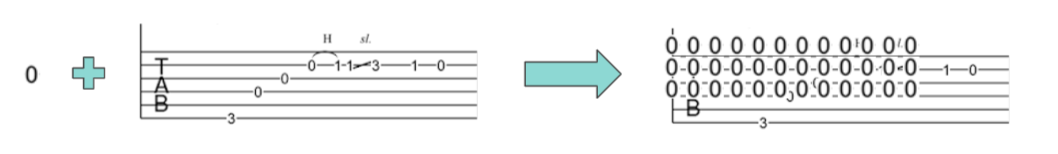
\includegraphics[width=0.8\linewidth]{method_1.png}
\end{center}
   \caption{Use small picture to find the exact number}
\label{fig:method_1}
\end{figure}

\begin{figure}[t]
\begin{center}
   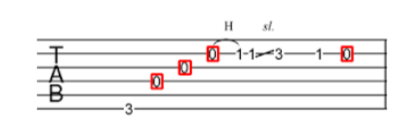
\includegraphics[width=0.8\linewidth]{method_2.png}
\end{center}
   \caption{Find the number 0 on lines}
\label{fig:method_2}
\end{figure}


The way we identify the score is to use the existing small pictures, and compare each small part of the entire score in a translation mode to see if there are similar images(Figure ~\ref{fig:method_1})(Figure ~\ref{fig:method_2}).

As for the method of identifying the position of each line of the hexagram, taking the first string as an example, we use the position with the largest number of "first encounters that are not white from top to bottom" as the first string.

\subsection{Pitch recognition}

We use aubio\cite{aubio_cite}, an open source code, for identification. The original topic was expected to use existing music for identification, but the results of the experiment were not good, so we changed to identify the input music in real time.

We use pyaudio\cite{pyaudio_cite} to receive the microphone signal from the computer. 
And we use aubio to determine the pitch of the input sound, then aubio will convert the sound to a MIDI Number.
Finally we will compare the MIDI number with the notes of the score.

%---------------------------------- --------------------------------------
\section{Experimental results}


We read multiple pictures of the staves at one time to identify the notes on the staves, that is, analyze the numbers and positions in the staves.

We divide the scores of each sheet into different lines and display them on the GUI. The user can play the guitar. After the program recognizes the correct pitch, the score on the GUI will automatically scroll.

\begin{figure}[t]
\begin{center}
   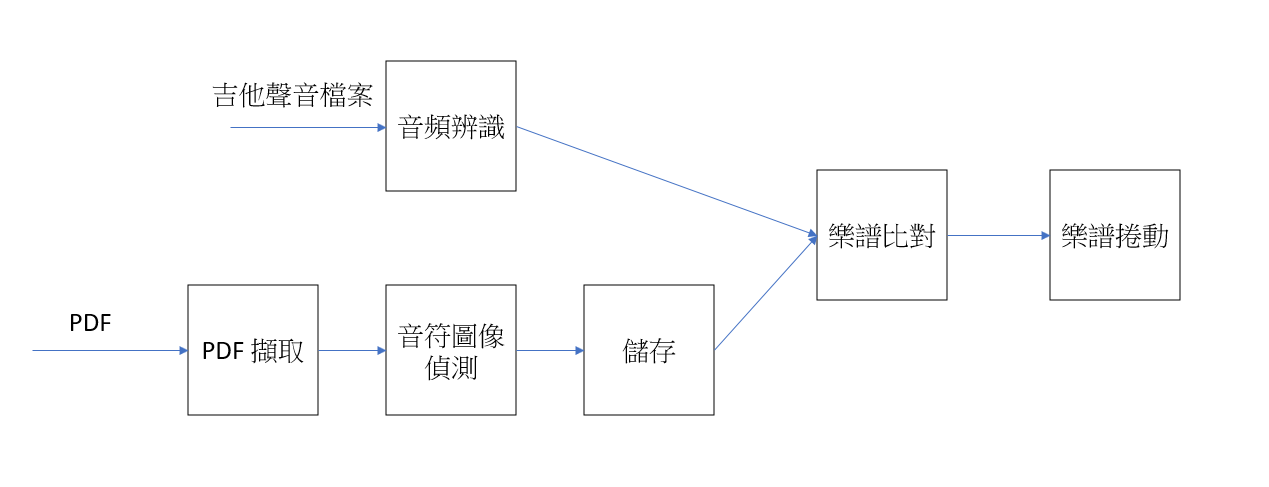
\includegraphics[width=0.8\linewidth]{system_framework.png}
\end{center}
   \caption{System Framework}
\label{fig:long}
\label{fig:system_framework}
\end{figure}

\subsection{System Framework}

Our experimental architecture is shown in the figure(Figure ~\ref{fig:system_framework}).
We read the tablature in PDF format and change them into png format. When inputting music later, we analyse the pitch. Once our system finds the input music matching the note on the tablature, it would scroll the tablature.


\subsection{GUI usage}

\begin{figure}[t]
\begin{center}
   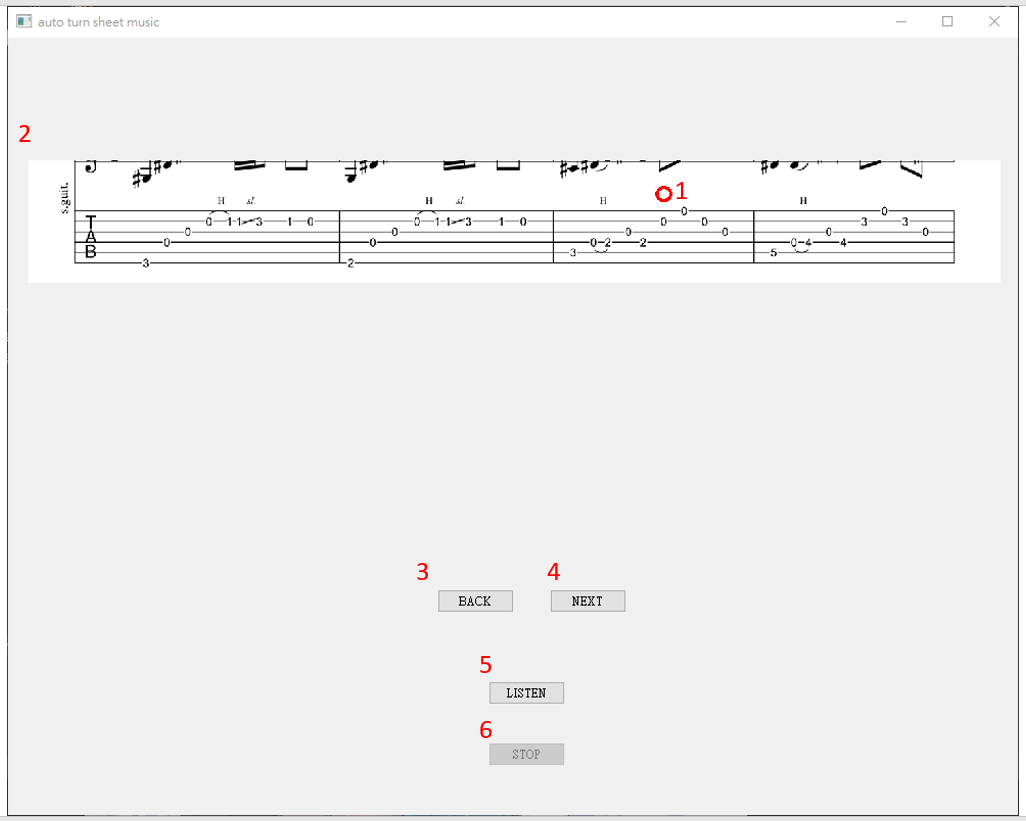
\includegraphics[width=0.8\linewidth]{gui.png}
\end{center}
   \caption{GUI}
\label{fig:gui}
\end{figure}

Following explains how to use the GUI (Figure ~\ref{fig:gui}).

\begin{description}
    \item 1. The red circle indicates which note is currently.
    \item 2. Show the current score.
    \item 3. Back the red circle one space.
    \item 4. Move the red circle one step forward.
    \item 5. Start to recognize the music mode.
    \item 6. Stop recognizing music mode.
\end{description}

When the red circle moves to the end of the score, it will automatically switch to the next page, and you can use the \emph{back} and \emph{next} buttons to manually move the position of the red circle.

Music recognition mode can recognize the input music and automatically change the position of the red circle.

%------------------------------------------------------------------------
\section{Conclusion}

When recognizing pitch, aubio uses \emph{confidence} as the basis for judging whether it is a note, but from the perspective of human hearing, some notes do not exist, or clearly exist but \emph{confidence} is much lower than other notes' \emph{confidence}.

Although our program can recognize music notes, it is still affected by other sounds, such as environmental sounds or human voices. In the pitch recognition part, we still have more room for improvement. 

We developed a software that can just listen to sound of guitar and scroll the tablature while it got a correct note.
{\small
    \bibliographystyle{ieee_fullname}
    \bibliography{egbib}
}

\end{CJK}
\end{document}
